\subsection{Task 5.1: Are shared trips cheaper?}
For each platform separately we compare reported matched shared trips ($Y/Y$) with non-shared trips ($N/N$). Passenger spending is the sum of the eight HVFHV monetary components used in Task 2; missing components are not set to zero and driver pay is excluded. We require completed trips, official directed OD zones, $0<\mathrm{trip\_miles}\leq100$, and positive finite spending. The audit CSV records the union and overlaps of exclusions. The reference for a shared trip is the mean non-shared spending in its same pickup month, directed OD, pickup hour, and weekday/weekend cell, requiring at least 30 reference trips. Within-zone OD pairs remain eligible.
Let $S_i$ be shared-trip spending and $\bar N_{c(i)}$ the non-shared mean in cell $c(i)$. We estimate $\hat\Delta=n^{-1}\sum_i(S_i-\bar N_{c(i)})$, weighting eligible shared trips equally. Negative values mean the reported matched trips cost less. We use a two-sided $t$ test of $H_0:\Delta=0$ with standard errors clustered by pickup date: $u_d=\sum_{i\in d}(S_i-\bar N_{c(i)}-\hat\Delta)$, $\widehat{SE}=\sqrt{D/(D-1)\sum_d u_d^2}/n$, and $D-1$ degrees of freedom. This accounts for same-day dependence; the confidence interval is $\hat\Delta\pm t_{0.975,D-1}\widehat{SE}$. Inference is conditional on the estimated non-shared reference means and does not propagate their sampling error; this especially limits the small Lyft sample. This is an observational comparison, not a causal discount estimate.
\begin{table}[htbp]\centering\small\caption{Task 5.1 passenger spending comparison; negative differences favor shared trips.}\label{tab:t5price}\begin{tabular}{llrrrrr}\hline Month & Platform & Shared $n$ & Coverage & $\hat\Delta$ (USD) & 95\% CI (USD) & $p$ \\ \hline
2026-04 & Uber & 85,060 & 33.3\% & -8.20 & [-8.85, -7.55] & 1.62e-21 \\
2026-04 & Lyft & 47 & 64.4\% & -16.26 & [-28.52, -4.00] & 0.0121 \\
2026-05 & Uber & 77,449 & 35.1\% & -8.14 & [-8.95, -7.33] & 3.53e-19 \\
2026-05 & Lyft & 38 & 55.9\% & -20.85 & [-35.44, -6.25] & 0.00843 \\
\hline\end{tabular}\end{table}
\begin{figure}[htbp]\centering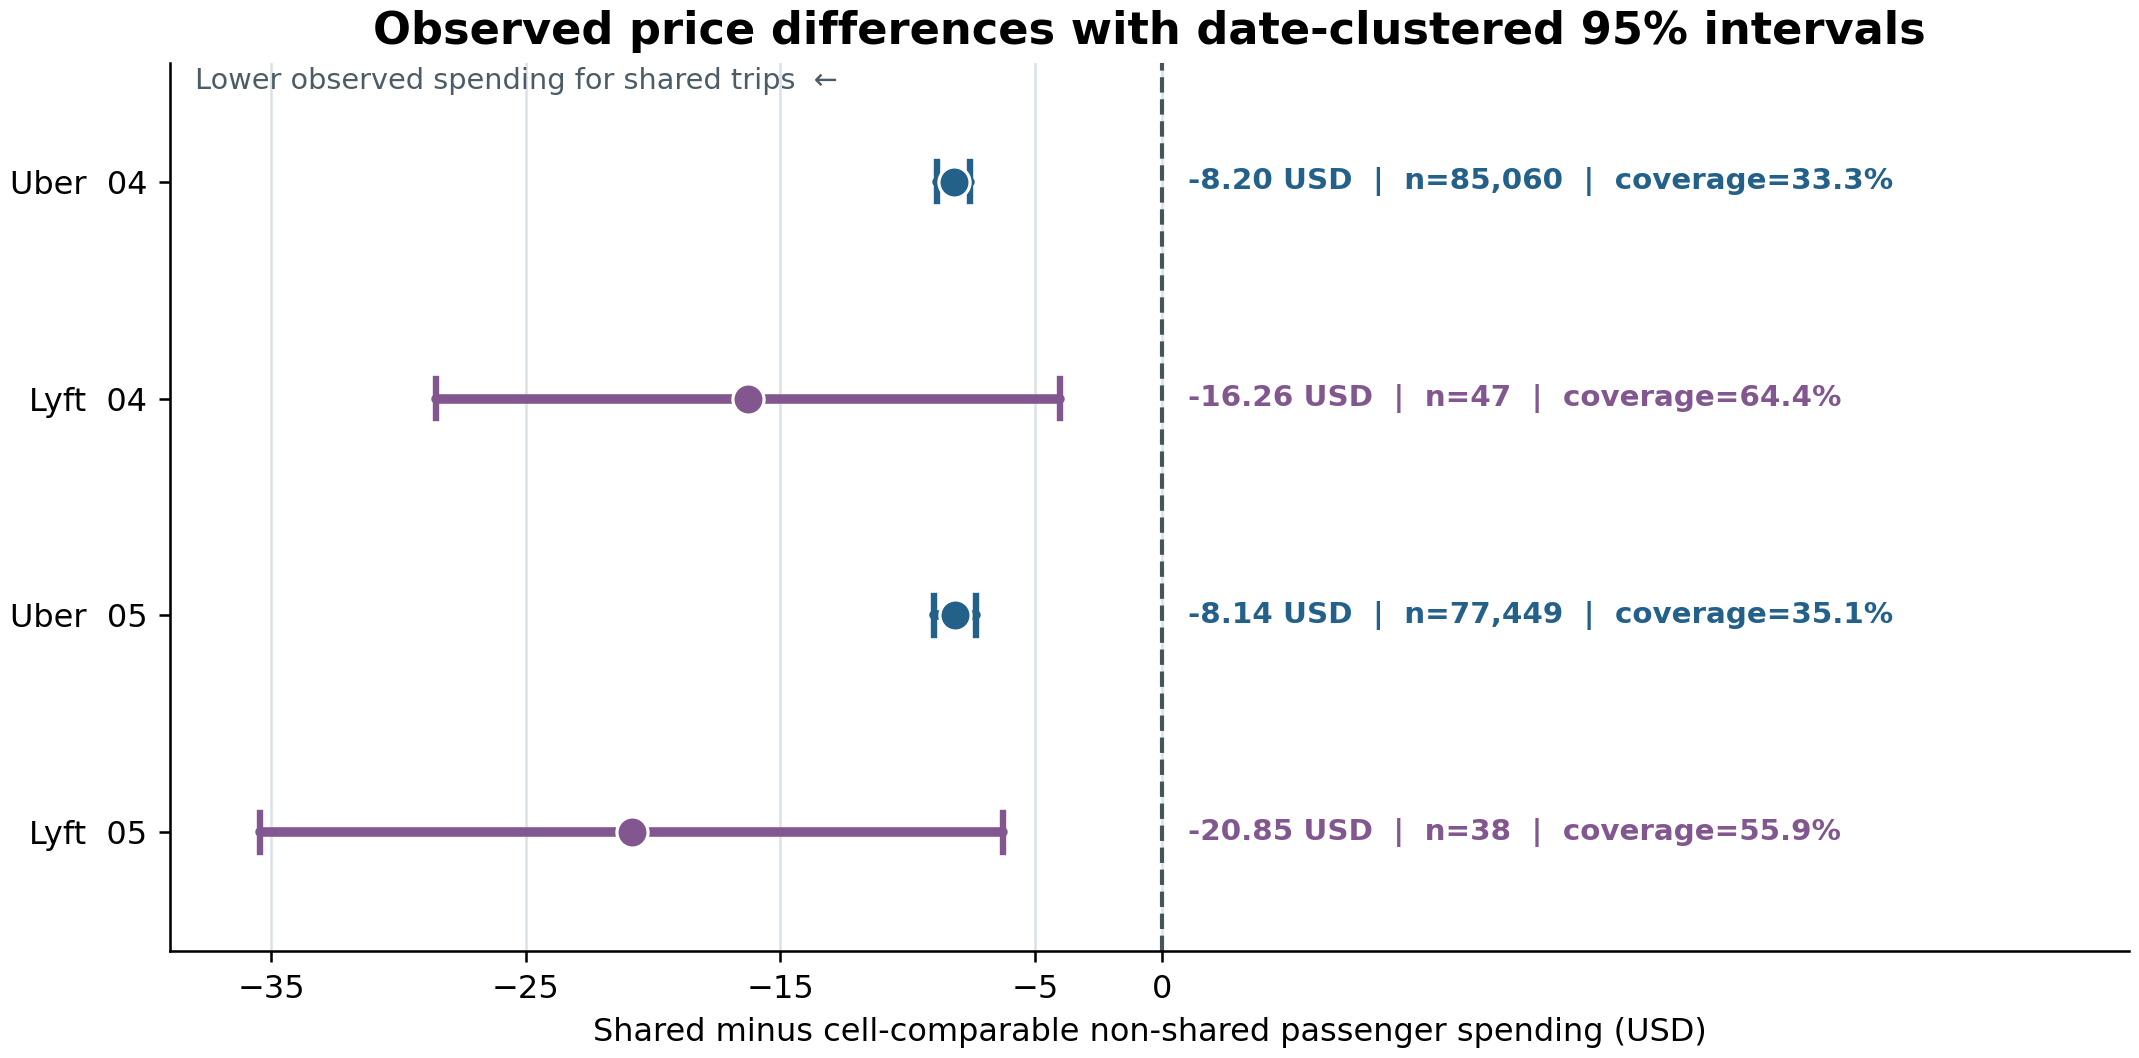
\includegraphics[width=.75\textwidth]{04_Results/Task_5/figures/price_differences.png}\caption{Shared minus cell-comparable non-shared spending, with day-clustered 95\% confidence intervals.}\label{fig:t5price}\end{figure}
For Uber in 2026-04, the comparable shared-trip mean is USD 20.67 versus USD 28.87 for its reference; the shared trips are USD 8.20 lower on average (-28.4\% relative to reference). The 95\% interval excludes zero; coverage is 85,060/255,346 eligible shared trips.
For Lyft in 2026-04, the comparable shared-trip mean is USD 39.41 versus USD 55.67 for its reference; the shared trips are USD 16.26 lower on average (-29.2\% relative to reference). The 95\% interval excludes zero; coverage is 47/73 eligible shared trips.
For Uber in 2026-05, the comparable shared-trip mean is USD 20.22 versus USD 28.36 for its reference; the shared trips are USD 8.14 lower on average (-28.7\% relative to reference). The 95\% interval excludes zero; coverage is 77,449/220,887 eligible shared trips.
For Lyft in 2026-05, the comparable shared-trip mean is USD 48.66 versus USD 69.51 for its reference; the shared trips are USD 20.85 lower on average (-30.0\% relative to reference). The 95\% interval excludes zero; coverage is 38/68 eligible shared trips.
Raw platform means are descriptive only: Lyft's shared mean is higher than its non-shared mean in both months, while its supported-cell differences are negative. Trip mix therefore matters. For Uber, the 10/30/50-reference-trip sensitivity estimates remain negative (April: USD -9.15/-8.20/-7.63; May: USD -9.15/-8.14/-7.45). Lyft's 10/30/50 estimates also stay negative but vary substantially with only 68--73 matched trips in each month; see the sensitivity CSV. The matched estimate is limited to supported cells and still permits unmeasured differences in exact endpoints, trip dates, route, passenger selection, promotions, and dynamic pricing. A reported $Y/Y$ flag does not verify the partner's identity or overlap duration. We use trip distance only to remove implausible records because pooling may itself change the driven distance. No causal discount is claimed.
\subsection{Task 5.2: Potentially shareable non-shared trips}
To estimate how many non-shared trips may have had a plausible sharing partner, we screen Uber and Lyft $N/N$ trips using a transparent zone-time rule. A trip is counted as potentially shareable if at least one other $N/N$ trip from the same platform and pickup month has the same directed OD pair and falls in the same pickup-time window. The main specification uses a 10-minute pickup window; 5- and 15-minute windows are reported as sensitivity checks. Completed trips must have official pickup/dropoff zones and $0<\mathrm{trip\_miles}\leq100$.
\begin{table}[htbp]\centering\small\caption{Task 5.2 potential shareability under the same-OD, 10-minute pickup-window rule.}\label{tab:t5potential}\begin{tabular}{llrrrr}\hline Month & Platform & Eligible $N/N$ & Potentially shareable & Share & Candidate pairs \\ \hline
2026-04 & Uber & 14,958,704 & 6,790,245 & 45.4\% & 9,356,742 \\
2026-04 & Lyft & 5,613,764 & 1,497,505 & 26.7\% & 1,361,286 \\
2026-05 & Uber & 14,962,744 & 6,701,182 & 44.8\% & 9,060,008 \\
2026-05 & Lyft & 6,766,606 & 1,915,041 & 28.3\% & 1,812,575 \\
\hline\end{tabular}\end{table}
\begin{figure}[htbp]\centering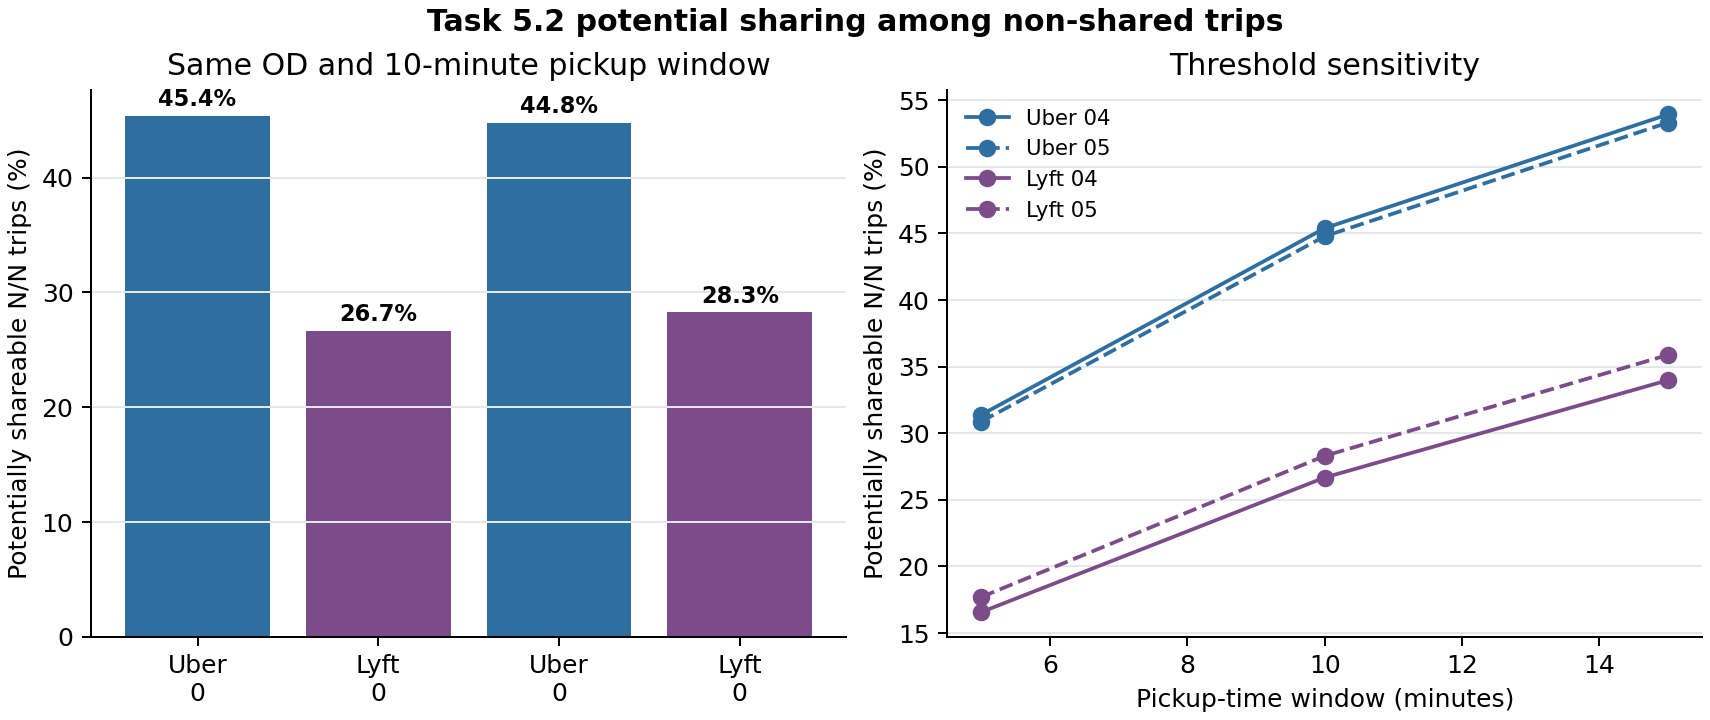
\includegraphics[width=.82\textwidth]{04_Results/Task_5/figures/potential_sharing.png}\caption{Potentially shareable non-shared trips under same-OD pickup-window rules. The left panel reports the 10-minute main rule; the right panel shows sensitivity to 5-, 10-, and 15-minute windows.}\label{fig:t5potential}\end{figure}
This screen suggests that a substantial share of non-shared completed trips had at least one coarse zone-time neighbor. Under the 10-minute rule, Uber has about 45.4\% in April and 44.8\% in May; Lyft has about 26.7\% and 28.3\%. The sensitivity table shows the expected monotonic pattern: wider pickup windows increase the potential-shareable count. These values should not be interpreted as trips that definitely could be pooled. Taxi Zones hide exact endpoints, the rule does not model waiting tolerance, detour cost, vehicle capacity, dispatch feasibility, or passenger willingness, and trips close to a time-window boundary may be misclassified. The result is therefore an upper-screening measure of latent co-occurrence in the non-shared trip stream, not a platform matching rate.

